\documentclass[11pt, a4paper]{article}
\usepackage{pdfpages}
\usepackage{parallel}
\usepackage[T2A]{fontenc}
%\usepackage{ucs}
\usepackage[utf8]{inputenc}
\usepackage[english,russian]{babel}
\usepackage{hyperref}
\usepackage{rotating}
\usepackage[inner=2cm,top=1.8cm,outer=2cm,bottom=2.3cm,nohead]{geometry}
%\usepackage{listings}
\usepackage{graphicx}
\usepackage{wrapfig}
\usepackage{longtable}
\usepackage{indentfirst}
\usepackage{array}
\usepackage{tikzsymbols}
\usepackage{soul}
\usepackage[ruled,vlined]{algorithm2e}
\usepackage{qrcode}
\counterwithout{figure}{section} 

\usepackage{url}
\makeatletter
\g@addto@macro{\UrlBreaks}{\UrlOrds}
\makeatother

\newcolumntype{P}[1]{>{\raggedright\arraybackslash}p{#1}}
\frenchspacing
%\usepackage{fixltx2e} %text sub- and superscripts
\usepackage{icomma} % коскі ў матэматычным рэжыме
%\PreloadUnicodePage{4}

\newcommand{\longpage}{\enlargethispage{\baselineskip}}
\newcommand{\shortpage}{\enlargethispage{-\baselineskip}}

\def\switchlang#1{\expandafter\csname switchlang#1\endcsname}
\def\switchlangbe{
\let\saverefname=\refname%
\def\refname{Літаратура}%
\def\figurename{Іл.}%
}
\def\switchlangru{
\let\saverefname=\refname%
\let\savefigurename=\figurename%
\def\refname{Литература}%
\def\figurename{Рис.}%
}
\def\switchlangen{
\let\saverefname=\refname%
\def\refname{References}%
\def\figurename{Fig.}%
}

\hyphenation{admi-ni-stra-tive}
\hyphenation{ex-pe-ri-ence}
\hyphenation{fle-xi-bi-li-ty}
\hyphenation{Py-thon}
\hyphenation{ma-the-ma-ti-cal}
\hyphenation{re-ported}
\hyphenation{imp-le-menta-tions}
\hyphenation{pro-vides}
\hyphenation{en-gi-neering}
\hyphenation{com-pa-ti-bi-li-ty}
\hyphenation{im-pos-sible}
\hyphenation{desk-top}
\hyphenation{elec-tro-nic}
\hyphenation{com-pa-ny}
\hyphenation{de-ve-lop-ment}
\hyphenation{de-ve-loping}
\hyphenation{de-ve-lop}
\hyphenation{da-ta-ba-se}
\hyphenation{plat-forms}
\hyphenation{or-ga-ni-za-tion}
\hyphenation{pro-gramming}
\hyphenation{in-stru-ments}
\hyphenation{Li-nux}
\hyphenation{sour-ce}
\hyphenation{en-vi-ron-ment}
\hyphenation{Te-le-pathy}
\hyphenation{Li-nux-ov-ka}
\hyphenation{Open-BSD}
\hyphenation{Free-BSD}
\hyphenation{men-ti-on-ed}
\hyphenation{app-li-ca-tion}

\def\progref!#1!{\texttt{#1}}
\renewcommand{\arraystretch}{2} %Іначай формулы ў матрыцы зліпаюцца з лініямі
\usepackage{array}

\def\interview #1 (#2), #3, #4, #5\par{

\section[#1, #3, #4]{#1 -- #3, #4}
\def\qname{LVEE}
\def\aname{#1}
\def\q ##1\par{{\noindent \bf \qname: ##1 }\par}
\def\a{{\noindent \bf \aname: } \def\qname{L}\def\aname{#2}}
}

\def\interview* #1 (#2), #3, #4, #5\par{

\section*{#1\\{\small\rm #3, #4. #5}}
\ifx\ParallelWhichBox\undefined%
    \addcontentsline{toc}{section}{#1, #3, #4}%
\else%
\ifnum\ParallelWhichBox=0%
    \addcontentsline{toc}{section}{#1, #3, #4}%
\fi\fi%

\def\qname{LVEE}
\def\aname{#1}
\def\q ##1\par{{\noindent \bf \qname: ##1 }\par}
\def\a{{\noindent \bf \aname: } \def\qname{L}\def\aname{#2}}
}

\newcommand{\interviewfooter}[1]{
\vskip 1em
\noindent \textit{#1}
}

\AtEndDocument{\vfill\centering \qrcode{https://github.com/fiowro/mouses/blob/main/\jobname.pdf}}

\switchlang{ru}
\begin{document}

\title{1984 "--- Siemens PC-D mouse}
\date{}
\maketitle
\selectlanguage{russian}
В 1984 году компания Siemens анонсировала персональный компьютер PC-D, работающий под управлением MS DOS, но аппаратно несовместимый с IBM PC. Этот компьютер был основан на процессоре Intel 80186, имел проприетарный монохромный графический адаптер с 12-дюймовым дисплеем, нестандартную клавиатуру иоперативную память объемом от 128 Кб до 1 Мб. Программное обеспечение включало MS DOS 2.11 и Windows 1.0, а также ряд офисных приложений и несколько простых игр \cite{wiki}. Годом позже список его дополнительных периферийных устройств пополнила двухкнопочная мышь (рис. \ref{fig:SiemensPCDPic}) \cite{blog}.

\begin{figure}[h]
    \centering
    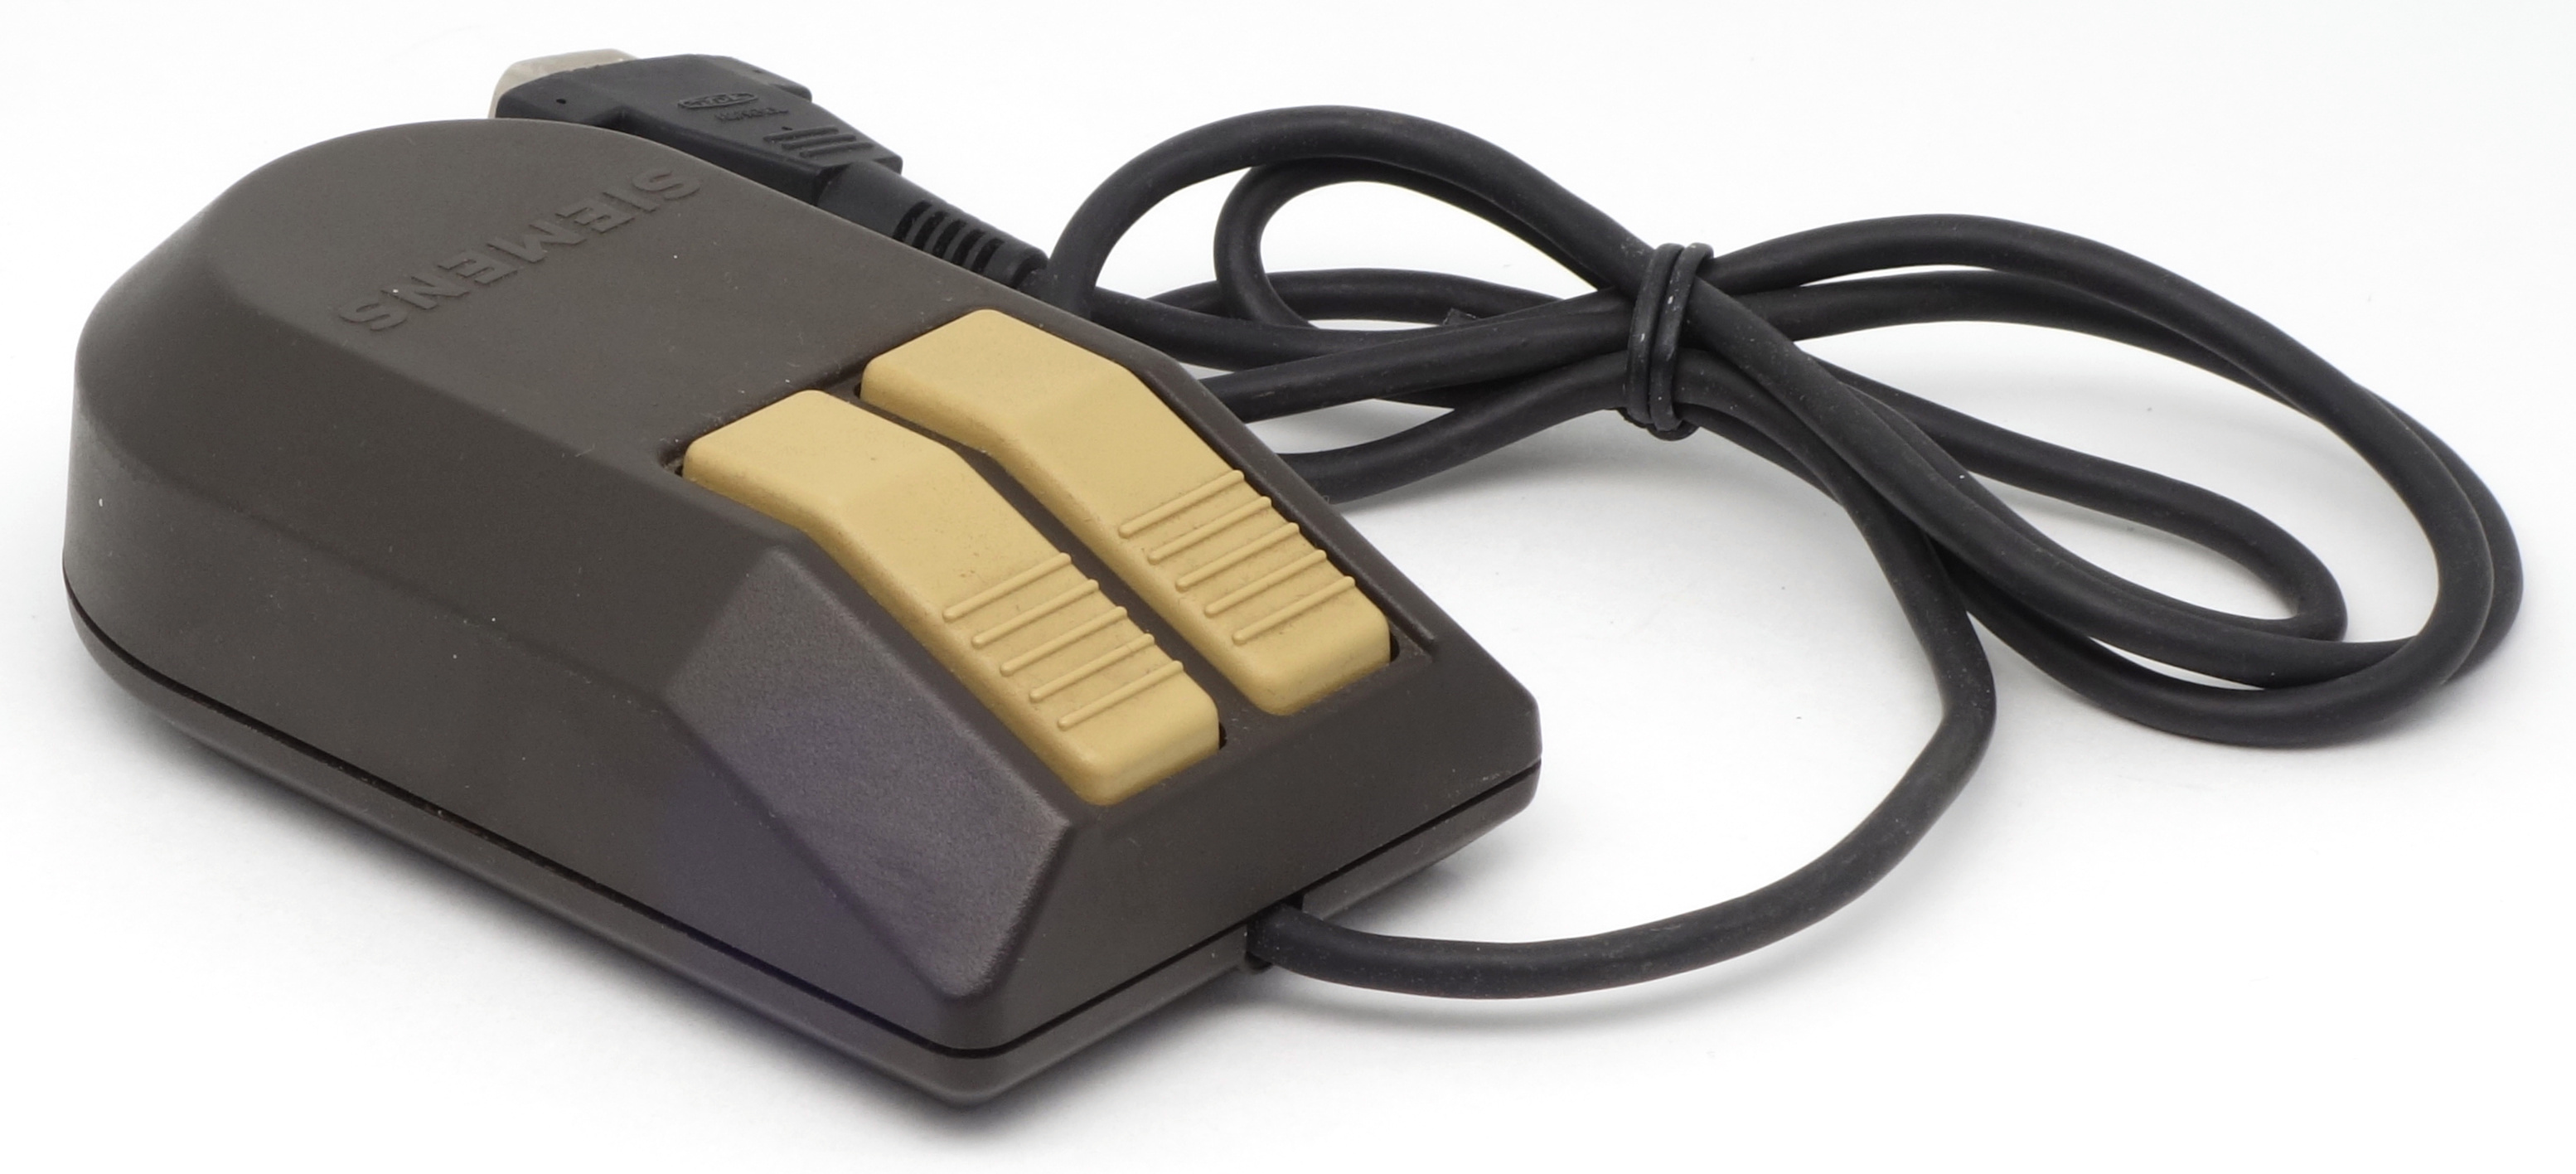
\includegraphics[scale=0.6]{1985_siemens_pcd_mouse/pic_30.jpg}
    \caption{Мышь Siemens PC-D Mouse}
    \label{fig:SiemensPCDPic}
\end{figure}

Как можно видеть (рис. \ref{fig:SiemensPCDTopBottom}), мышь выполнена в контрастной черно-бежевой цветовой схеме (однако встречаются также фотографии данной мыши в однотонном бежевом корпусе). Сверху присутствуют две контрастные кнопки и название компании; в целом корпус имеет сложную рубленую форму и не содержит дополнительных элементов. Нижняя часть содержит прорезиненный шар и фиксирующее кольцо, которое можно сдвинтуть в сторону, чтобы извлечь шар для чистки мыши. Вокруг фиксирующего кольца наблюдается контрастная кольцеобразная накладка из низкофрикционного материала, являющася отличительной чертой многих мышей 80-х годов, разработанных в Японии.

\begin{figure}[h]
    \centering
    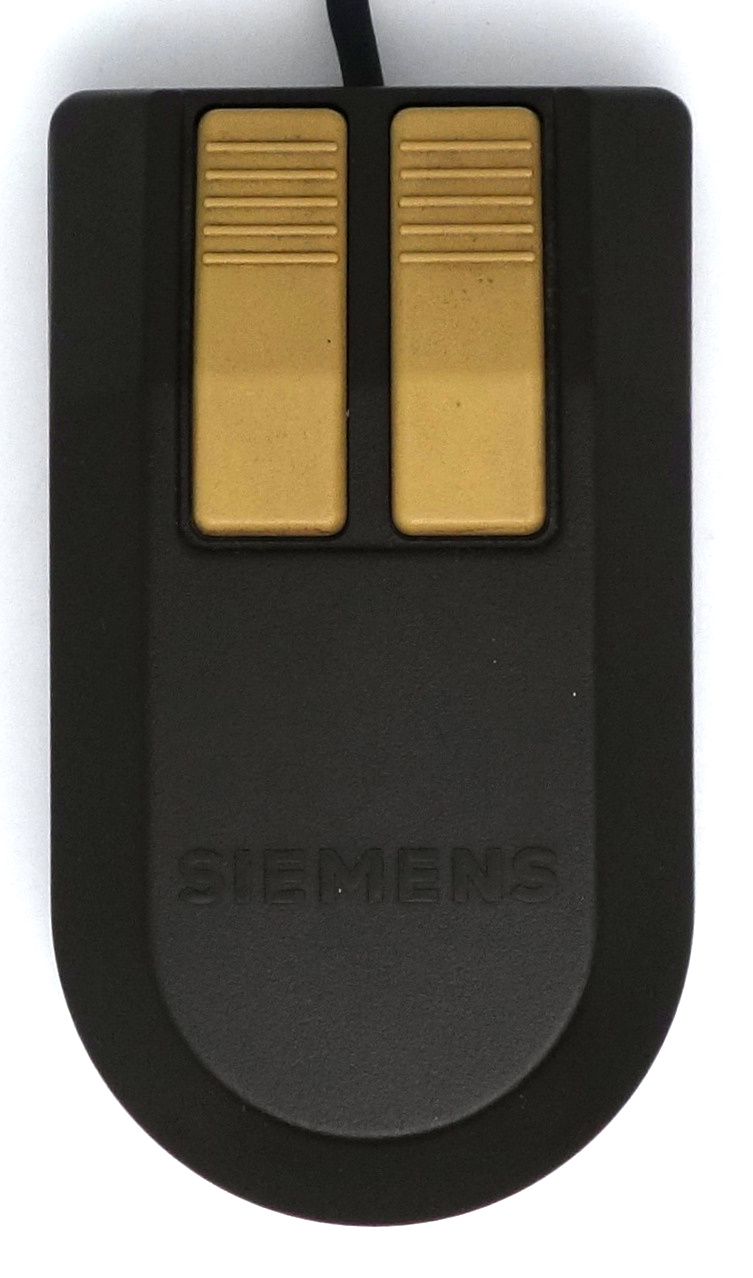
\includegraphics[scale=0.45]{1985_siemens_pcd_mouse/top_30.jpg}
    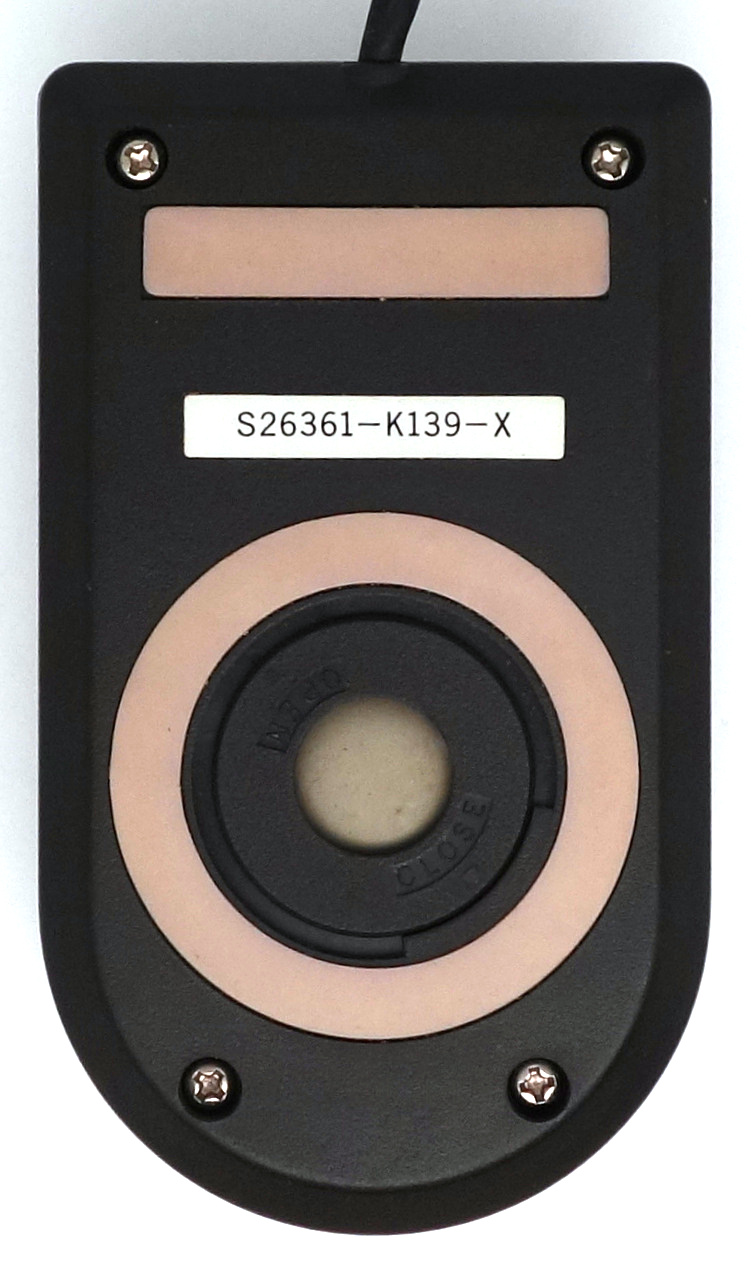
\includegraphics[scale=0.45]{1985_siemens_pcd_mouse/bottom_30.jpg}
    \caption{Siemens PC-D Mouse, вид сверху и снизу}
    \label{fig:SiemensPCDTopBottom}
\end{figure}

В плане размера манипулятор представляет собой типичное для 80-х годов оптомеханическое устройство управления курсором (рис. \ref{fig:SiemensPCDSize}).

\begin{figure}[h]
    \centering
    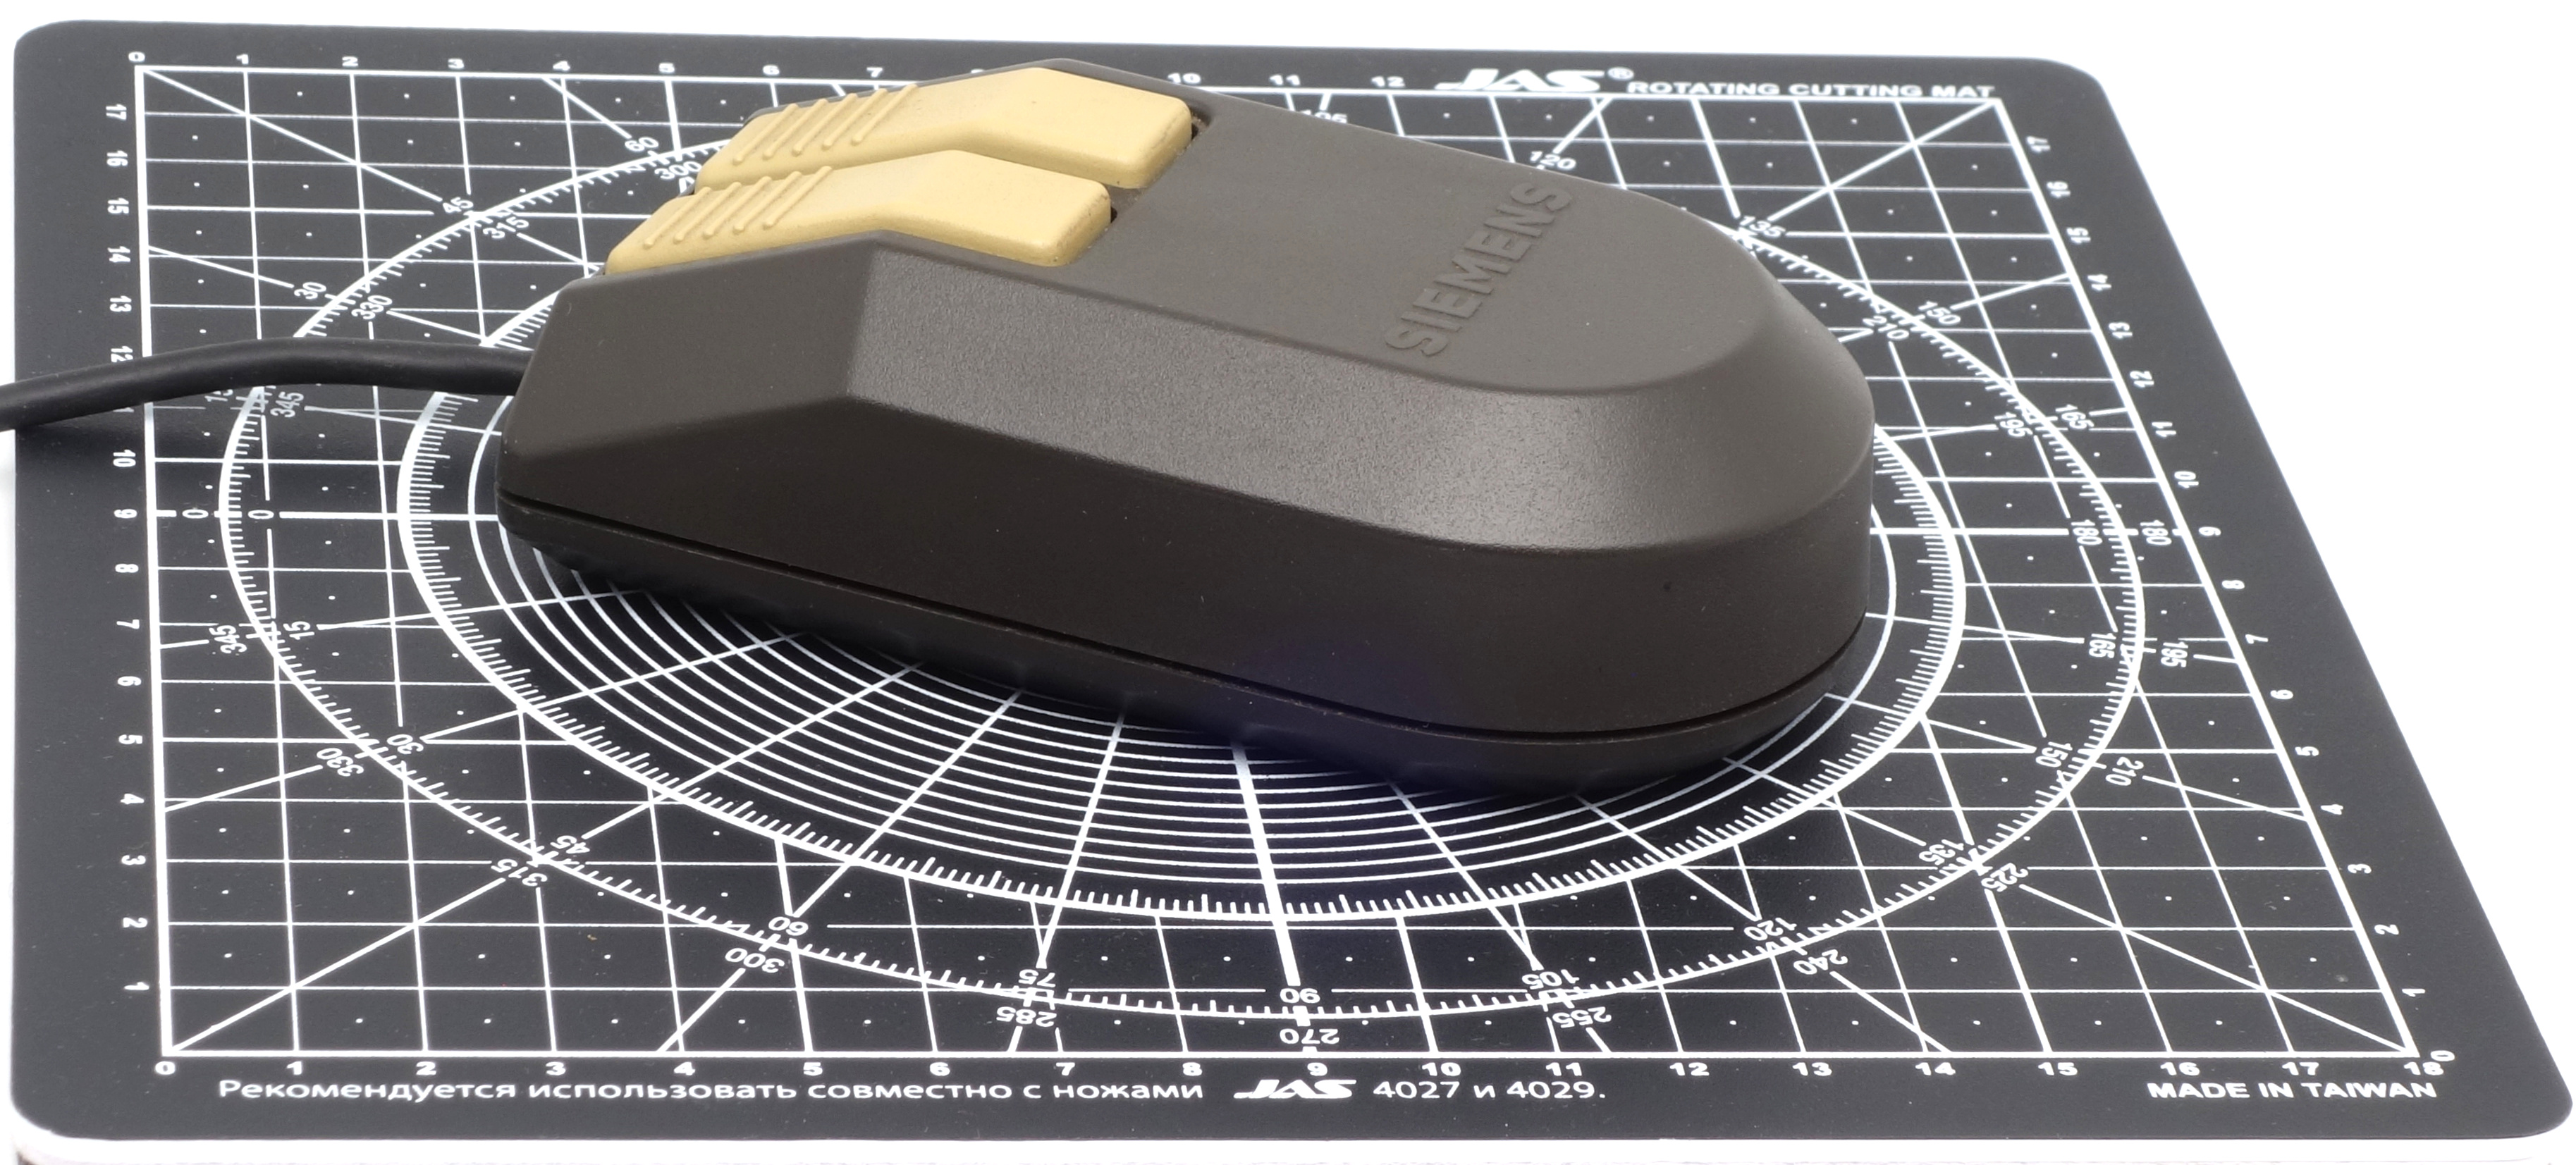
\includegraphics[scale=0.42]{1985_siemens_pcd_mouse/size_30.jpg}
    \caption{Изображение Siemens PC-D Mouse на размерном коврике с шагом сетки 1~см}
    \label{fig:SiemensPCDSize}
\end{figure}

В плане эргономики и во внешнем виде PC-D Mouse прослеживается ярко выраженный индустриальный дизайн. При этом большое количество углов и плоских граней отчасти компенсируется закругленными стыками граней. Кнопки расположены на наклонной передней грани и заходят на верхнюю стенку тела (рис. \ref{fig:SiemensPCDHand}). По рекомендации производителя их следует нажимать средним и безымянным пальцем, придерживая мышь с боков указательным пальцем и мизинцем \cite{manual}.

\begin{figure}[h]
    \centering
    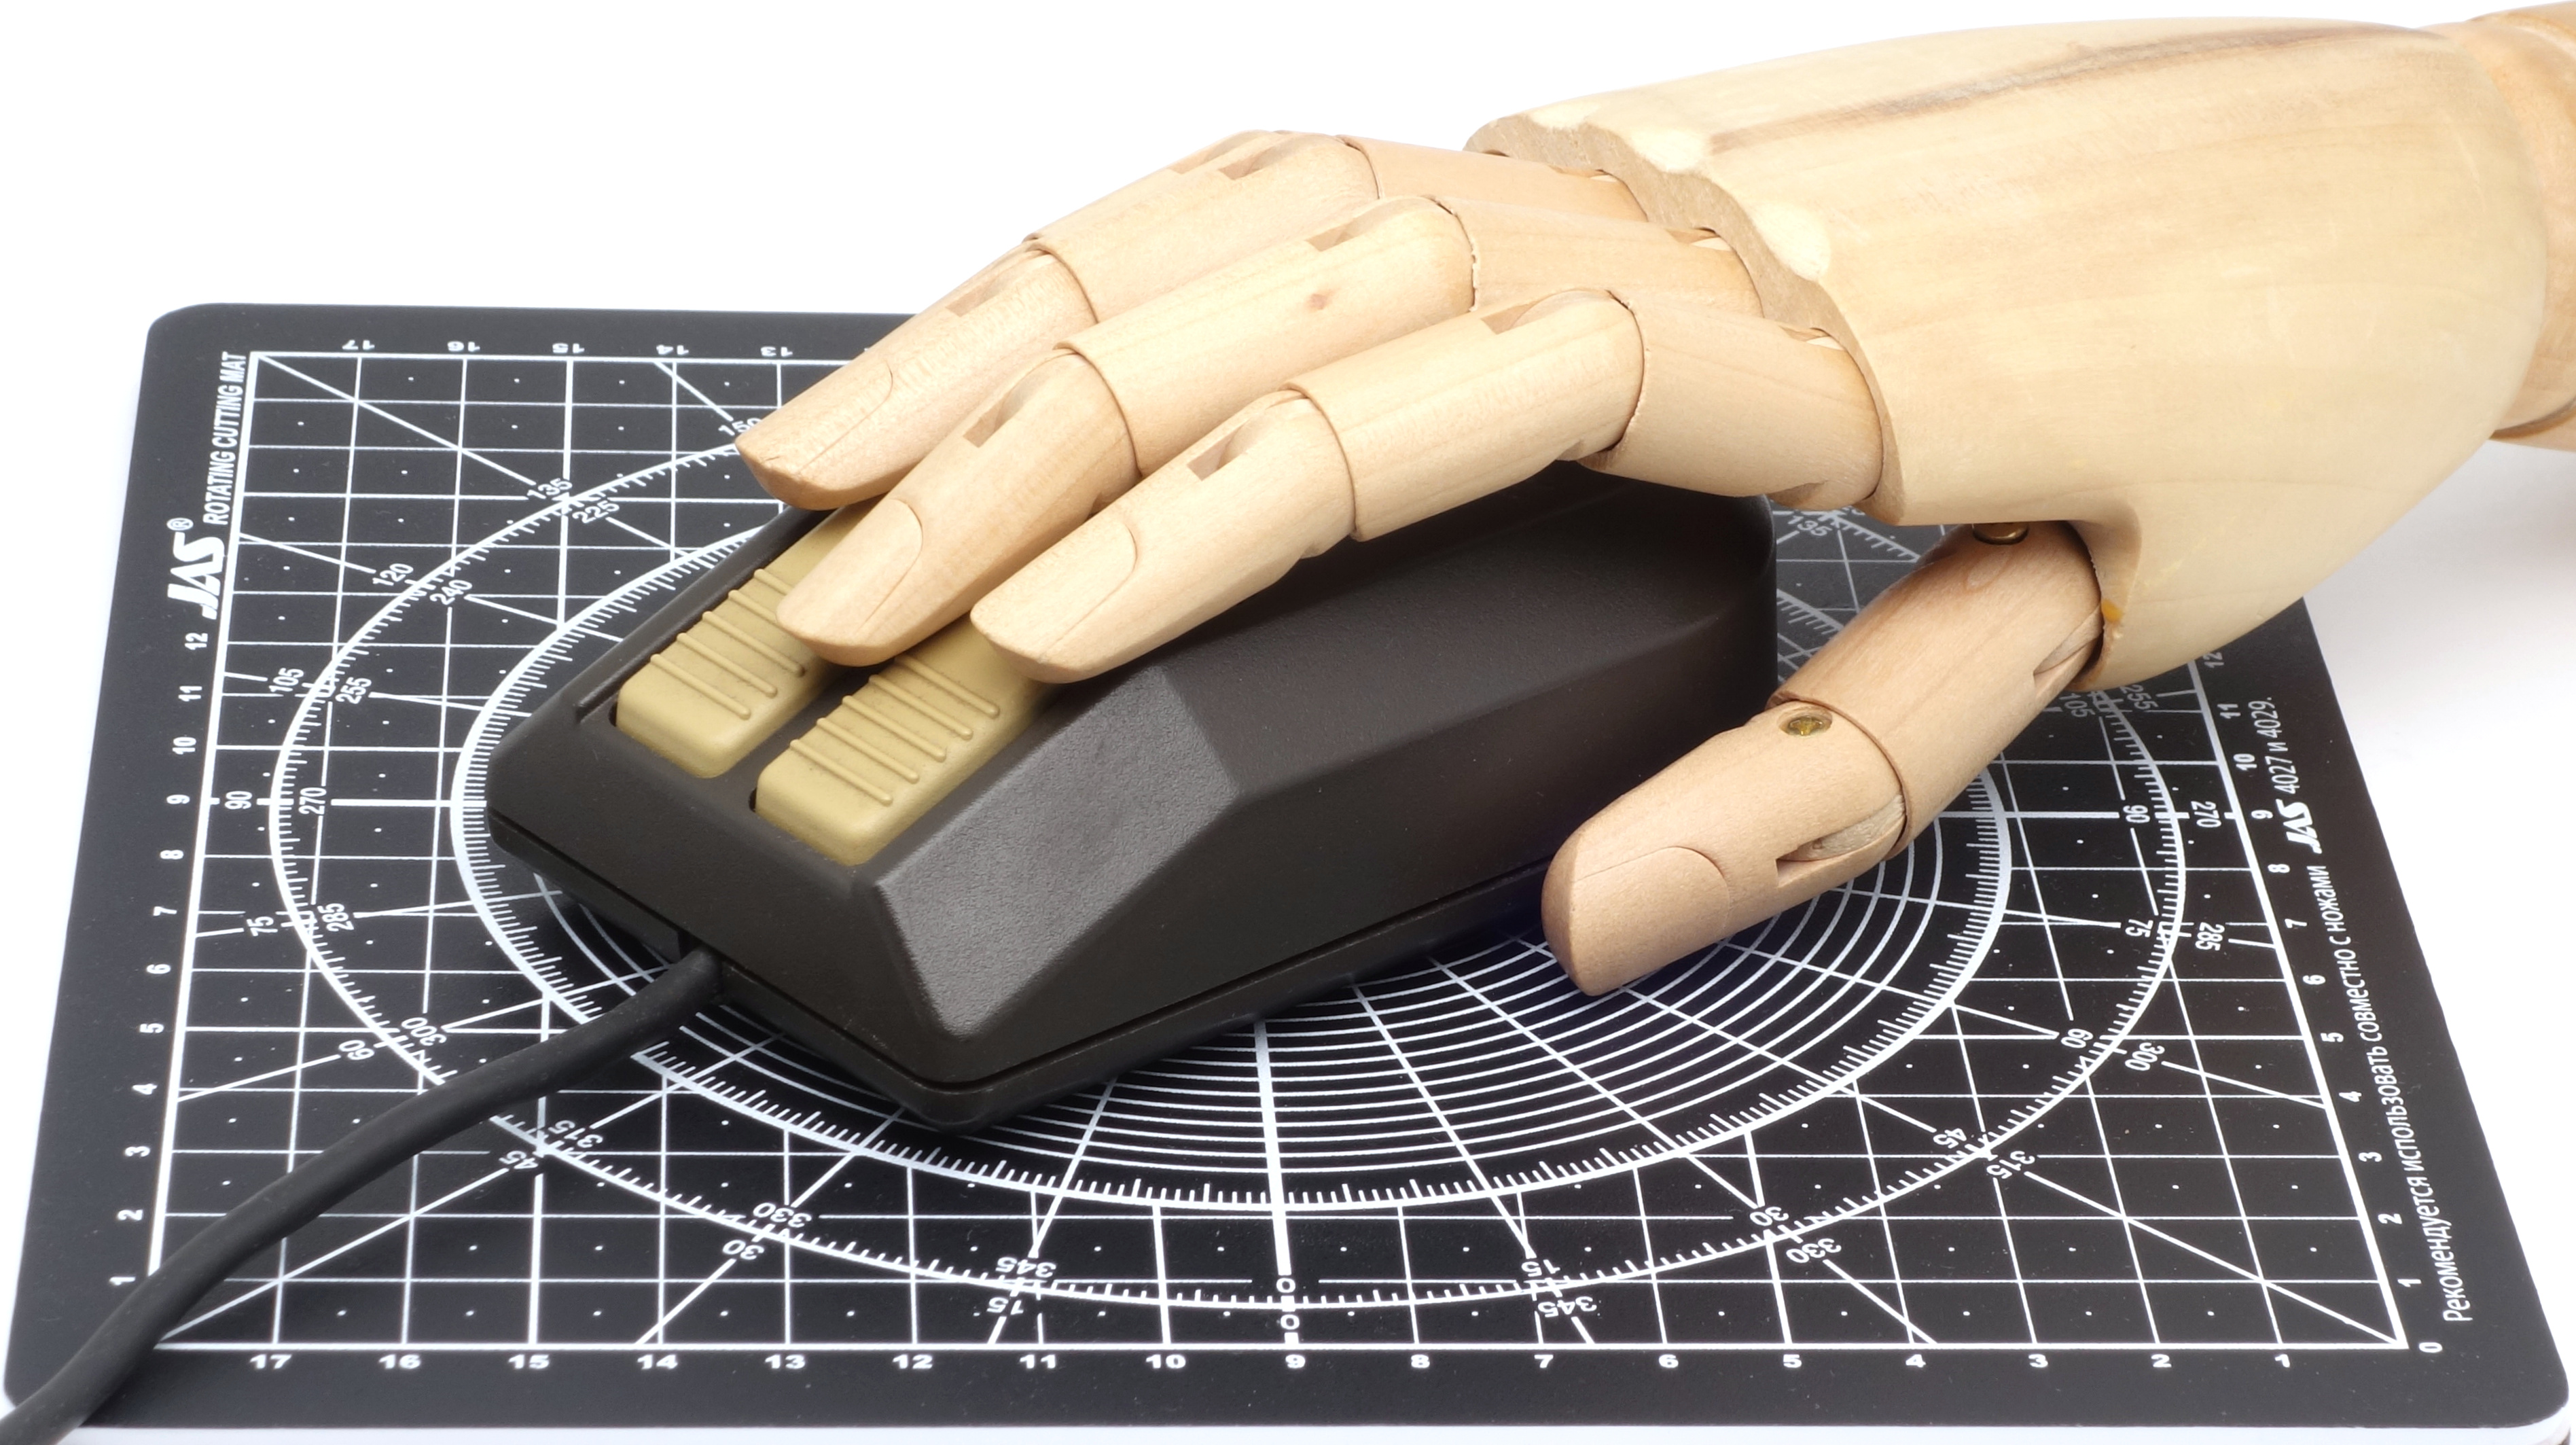
\includegraphics[scale=0.42]{1985_siemens_pcd_mouse/hand_30.jpg}
    \caption{Изображение Siemens PC-D Mouse с моделью руки человека}
    \label{fig:SiemensPCDHand}
\end{figure}

Внутреннее устройство Siemens PC-D Mouse показано на рис. \ref{fig:SiemensPCDInside}, что позволяет классифицировать мышь как устройство с опто-механическим энкодером, изготовленное в Японии.

\begin{figure}[h]
    \centering
    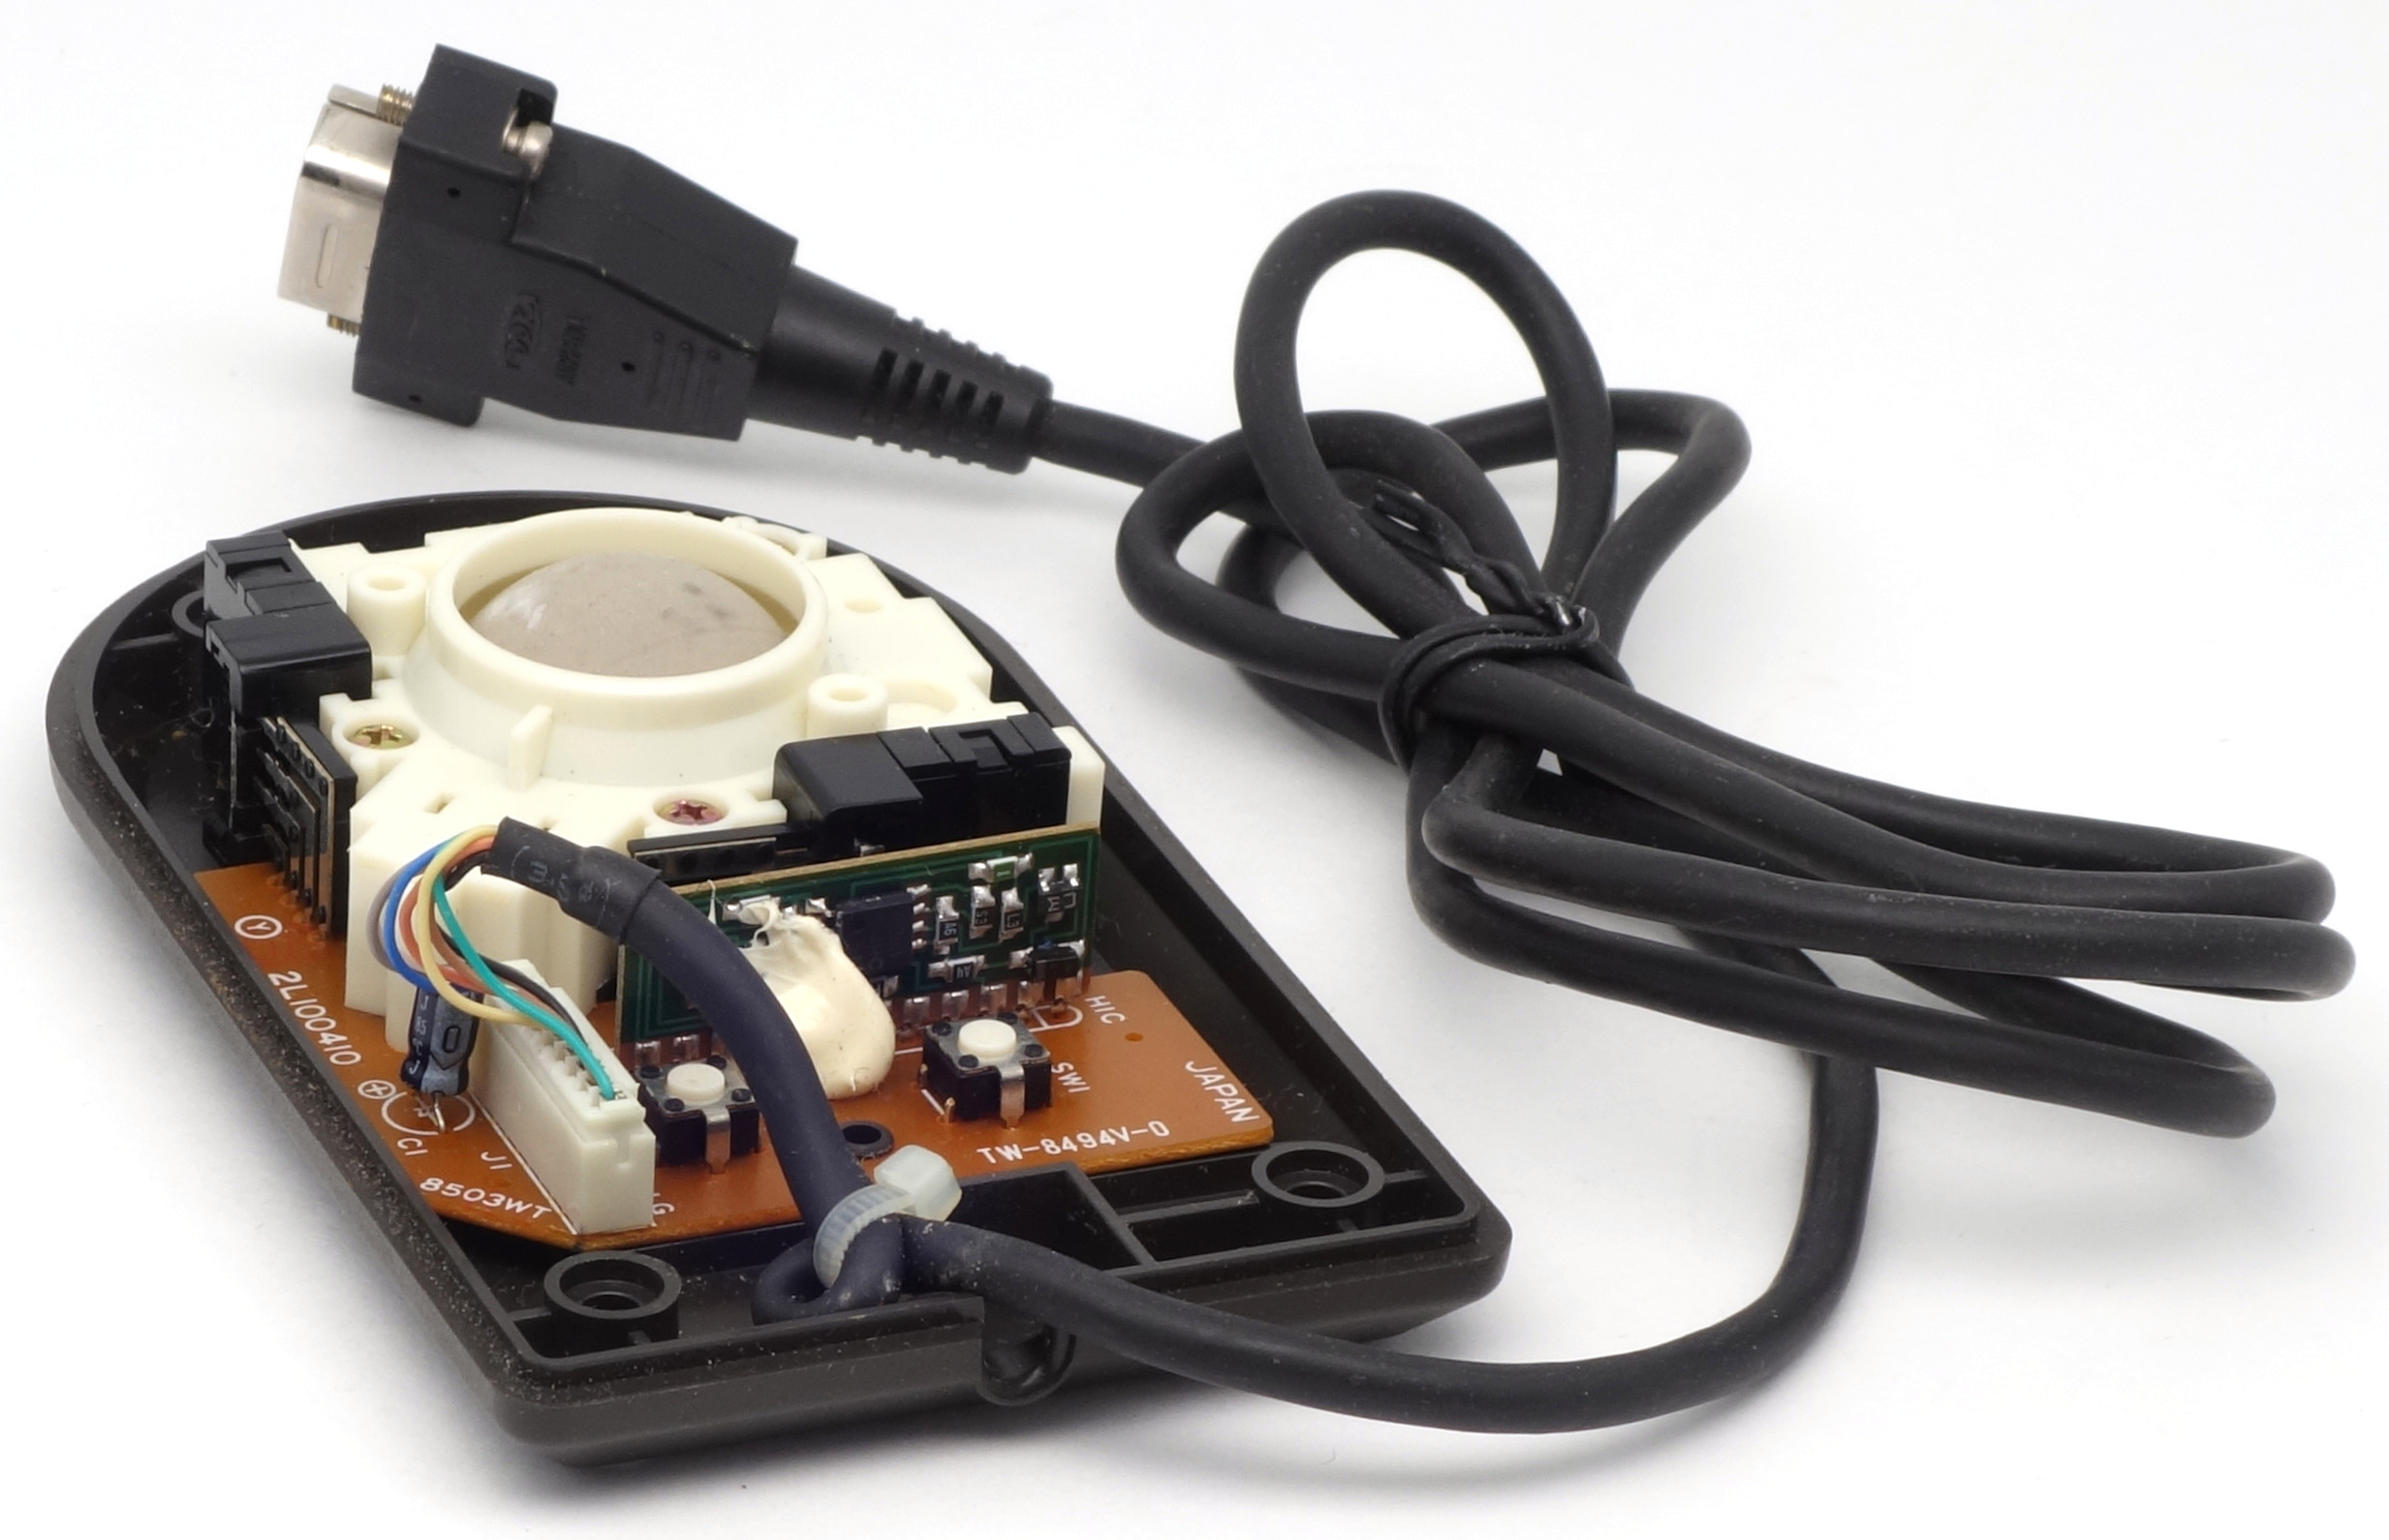
\includegraphics[scale=0.8]{1985_siemens_pcd_mouse/inside_30.jpg} 
    \caption{Siemens PC-D Mouse в разобранном состоянии}
    \label{fig:SiemensPCDInside}
\end{figure}

Очевидно, реальным изготовителем мыши была японская компания Alps, часто выступавшая подрядчиком в разработке мышей по заказу других фирм (услугами Alps в частности пользовались такие компании, как IBM, Microsoft, NeXT, Intergraph). Alps обычно изготавливала для каждого заказчика дизайн мыши с уникальной формой корпуса и расположением кнопок, но использовала одно и то же конструктивное исполнение в нескольких устройствах. В частности, данная мышь совпадает (включая нижнюю часть корпуса, узел оптомеханического преобразования на основе закрытых энкодеров, печатную плату с радиоэлементами) с оригинальной мышью компьютеров NeXT, выпускавшихся с 1988 года, и с мышью компьютеров Intergraph InterPro 2020, появившихся на рынке в 1992 году.

\begin{thebibliography}{9}
\bibitem {wiki} Siemens PC-D -- Wikipedia \url{https://en.wikipedia.org/wiki/Siemens_PC-D}
\bibitem {blog} Der PC von Siemens. Heinz Nixdorf MuseumsForum \url{https://blog.hnf.de/der-pc-von-siemens/}
\bibitem {manual} MAUS. Bedienelement für Siemens PC-D. Anwendungsbeschreibung. Ausgabe Dezember 1985. \url{https://github.com/fiowro/mouses/blob/main/source/OCR/PC-D_mouse.pdf}
\end{thebibliography}
\end{document}
